\documentclass[../main.tex]{subfiles}
\begin{document}
%\chapter{Finto}
%\newpage
\setchapterimage[6.5cm]{images/Polar_stereographic_projections}
\setchapterpreamble[u]{\margintoc}
\chapter[Manifolds]{Manifolds\footnotemark[0]}
\labch{manifold}
\section[The extrinsic viewpoint]{Introduction: The extrinsic viewpoint}
Let us anticipate that 
\[
\text{\parbox{4 cm}{\centering n-dimensional \\[-4pt]  (smooth) manifold}}\underset{\mathclap{\tikz \node {$\uparrow$} node [below=1ex] {\footnotesize circa};}}{\simeq}\text{\parbox{4 cm}{\centering n-dimensional \\[-4pt]  (smooth) surface}}
\]
We can visualize a 2-dimensional smooth surface, for example the thorus in \reffig{Torus}, represented as a subset of $\mathbb{R}^3$. 
\begin{figure}[H]
	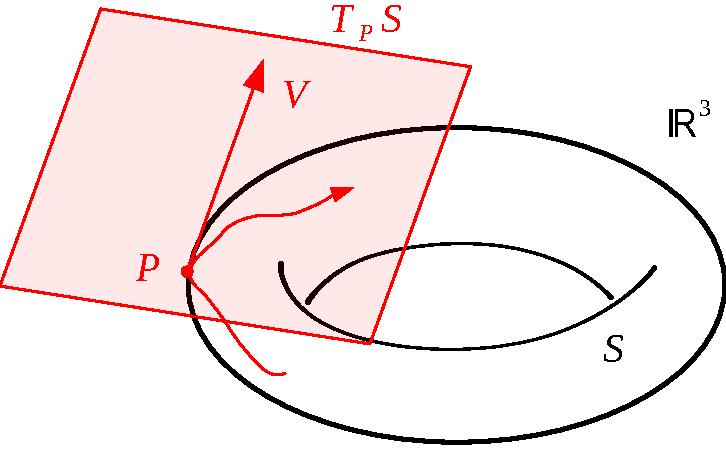
\includegraphics[width=1\textwidth]{images/Toro.pdf}
	\caption[Torus]{Representation of a 2-dimensional torus in $\mathbb{R}^3$ with the point $P$ and its tangent vector $v$.}
	\labfig{Torus}
\end{figure}
The relevant thing is that we can consider smooth path
\[
\begin{split}
\gamma:(-1,1)&\xrightarrow{C^\infty} S\subseteq\mathbb{R}^3\\
t &\mapsto \gamma(t)
\end{split}
\]
with $\gamma(0)=P$. Once we defined this path, we can consider its velocity (the derivative with respect to this pseudo time), in particular the velocity at time $0$ will be a tangent vector to the surface at the point $P\in S$
\[
\frac{d}{dt}\gamma(t)\Bigr|_{\substack{t=0}}\equiv\Dot{\gamma}(0)=\underset{\mathclap{\tikz \node {$\uparrow$} node [below=1ex] {\footnotesize Tangent vector at the point $p\in S$};}}{V}\in\mathbb{R}^3
\]
Now with the notion of tangent vector, we can define what is a tangent space.
\begin{definition}[Tangent space]\index{Tangent space}
The tangent space to $S$ at $P\in S$ is
\begin{align*}
V_P=T_P S=&\left\{V\in \mathbb{R}^3: V=\Dot{\gamma}(0)\right.\\ 
&\left.\textrm{ for some path } \gamma: (-1,1)\xrightarrow{C^\infty} S \mbox{ with } \gamma(0)=P\right\}
\end{align*}
\end{definition}
%1:28:00
As a vector space we can consider its dual\marginnote{We will see later that, for example, in classical mechanics velocities are identified with elements of the tangent space, while momenta are naturally identified with elements of the cotangent space.}
\begin{definition}[Cotangent space]\index{Cotangent space}
The cotangent space is the dual of the tangent space
\[
V_P^*=\begin{Bmatrix}\alpha:V_P \rightarrow \mathbb{R} \ \mbox{ linear}\end{Bmatrix}=T_P^* S
\]
\end{definition}
But there is something unpleasant in all the description we have done: the embedding in an ambient space. Everything we said it is correct, but it might depend on the fact that our 2-dimensional torus is embedded in $\mathbb{R}^3$ and someone else could decide to embed it in $\mathbb{R}^4$. The approach we described is called the \textbf{extrinsic} viewpoint and it traces back to: Gauss = Gauß (\underline{credits}), who realised that there are some properties of surfaces which depends on the embedding: \textbf{extrinsic} properties.
\section[The intrinsic viewpoint]{Introduction: The intrinsic viewpoint}\marginnote{\underline{Credits:} Gauss, Riemann, ...,  Weyl}
Gauß himself realized that there were some properties of surfaces, that are independent of the embedding in a larger space. This properties are called \textbf{intrinsic} properties, hence it would be nice to have an intrinsic viewpoint: define an n-dimensional (smooth) surface, without the ambient space.\sidenote{Why should we be interested in this generalization? Because we are physicist and if we want to describe space-time, we need an intrinsic viewpoint. Even if our friend from string theory told us that our 4-dimensional space-time is just a sub-manifold of a ten(eleven)-dimensional larger object. It might be true or false, but in this way the problem is just postponed: then we have to describe this eleven-dimensional geometric object with some embedding. You are forced to invoke something that is non-physical to describe something that is physical.} The idea comes from cartography\sidenote{We all learned at school that there is no cartographic map of the all surface of Earth, but locally we can represent it by something flat: a piece of paper.}
\[
\textrm{\underline{Keywords:} local chart, atlas, } \dots \textrm{(cartography)}
\]
where we have a set $\mathbf{M}$ and different subsets of $\mathbf{M}$ described in terms of local charts. Let us take the example in \reffig{Charts}
\begin{itemize}
    \item We take a subsets $u$ of a set $\mathbf{M}$;
    \item in the region of a subset, the subset is well described by a local chart (a page in our atlas), which are maps from an open subsets of $\mathbb{R}^n$ to $u$:
    \[
    \varphi^{-1}(w)\to\mathbf{M}
    \]
    which give to every point $P$ a set of coordinates. Unless the set is flat, there will be no chart which covers the all $\mathbf{M}$. The problem is that if we have many, we could have a problem of compatibility (see \vrefdef{comp-charts}).
    \item The point $P$ can be also contained in another subset $\tilde{u}$ and described by another pair of coordinated $(\tilde{x}_1, \tilde{x}_2)$
    \item Therefore, in the intersection of the two subsets we will have a smooth change of coordinates 
\end{itemize} 
\begin{figure}[H]
	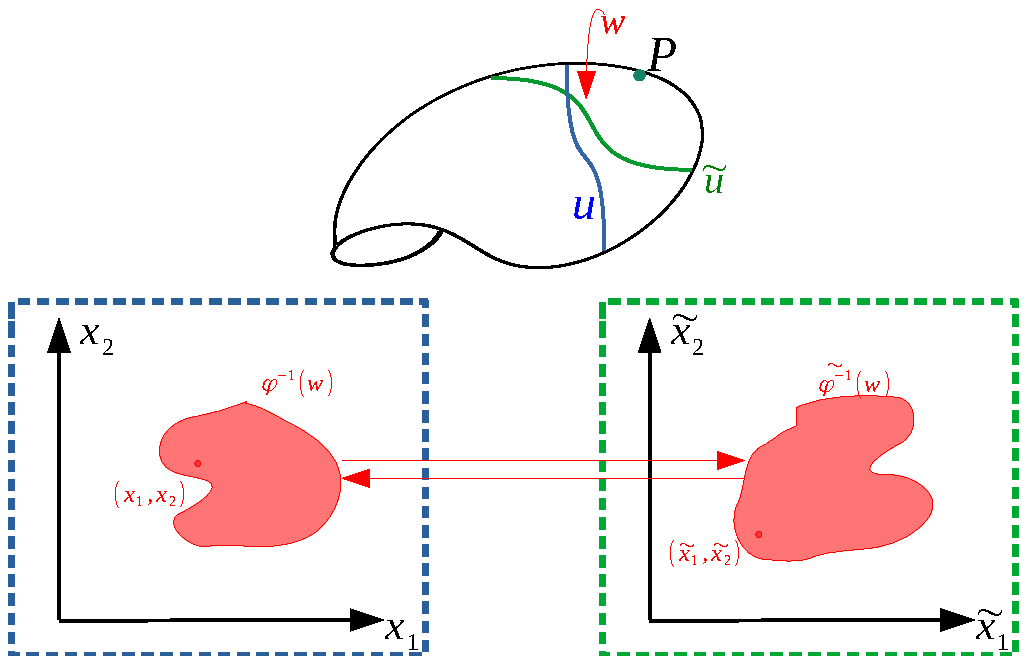
\includegraphics[width=1\textwidth]{images/Charts.pdf}
	\caption[Charts]{Representation of the change of coordinates from two different subsets $u$ and $\tilde{u}$ of a 2-dimensional manifold $M$.}
	\labfig{Charts}
\end{figure}
The main message is that there is an intrinsic mathematical object, the point $P$, expressed in terms of the pair $(u,\varphi)$, called \textbf{local chart}
\[
\text{\parbox{2 cm}{\centering chart \\[-4pt]  $(u,\varphi)$}}\longleftrightarrow\text{\parbox{2 cm}{\centering intrinsic \\[-4pt]  object}}\longleftrightarrow\text{\parbox{2 cm}{\centering local chart \\[-4pt] $(\tilde{u},\tilde{\varphi})$}}
\]
\[
\varphi(x_1,x_2)=P=\Tilde{\varphi}(\Tilde{x_1},\Tilde{x_2})
\]
{\fontencoding{U}\fontfamily{futs}\selectfont\char 66\relax} The key idea is that we have to impose that the local \textbf{change of coordinates must be \underline{\underline{smooth}}}!.\marginnote[2mm]{\href{http://www.thelatinlibrary.com/justinian/institutes2.shtml\#ii:vii}{(Giustiniano, Institutiones, libro II, 7, 3)}}
\[
\textrm{Motto: \  <<\href{https://it.wikipedia.org/wiki/Nomen_omen}{NOMINA SVNT CONSEQVENTIA RERVM}>>}
\]
%%%%%%%%%%%%%%%%%%%%%%%%%%%%%%%%%%%%%%%%%%%%%
\section{Precise definitions}
\paragraph{Mapping \sidecite{ferrari2020general}}
\begin{marginfigure}[17mm]
	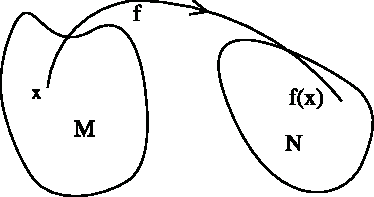
\includegraphics{images/mappa_vettoriale.pdf}
	\caption[Mapping from $\mathbf{M}$ to $\mathbf{M}$]{Mapping from $\mathbf{M}$ to $\mathbf{N}$. Figura presa da \cite{ferrari2020general}.}
	\labfig{mappa}
\end{marginfigure}
\begin{definition}[Map - Mappa]
A map\index{Map} $f$ from a space $\mathbf{M}$ to a space $\mathbf{N}$ is a rule which associates en element $\mathbf{x}$ of $\mathbf{M}$ to a unique element $\mathbf{y}=f(\mathbf{x})$ of $\mathbf{N}$. The space $\mathbf{M}$ and $\mathbf{N}$ need not to be different.
\end{definition}
It is also said that $f$ maps a points $\mathbf{x} \in \mathbf{M}$ \textit{into} a point $f(\mathbf{x}) \in \mathbf{N}$. The statement “$f$ maps $\mathbf{M}$ into $\mathbf{M}$” is indicated as \[f : \mathbf{M} \rightarrow  \mathbf{N}\]
In addition, $f$ maps a particular element $\mathbf{x} \in \mathbf{M}$ into $\mathbf{y} \in \mathbf{N}$; the mapping is indicated as
\[
f : \mathbf{x} \mapsto  \mathbf{y}
\]
\begin{marginfigure}
	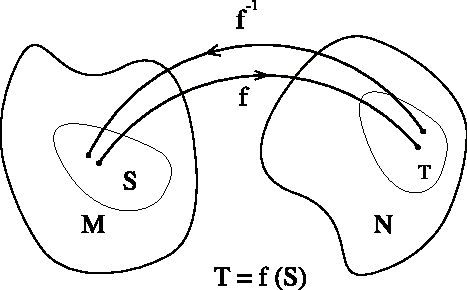
\includegraphics{images/immagine_e_inversa_mappa.pdf}
	\caption[Image and inverse image of a mapping.
]{Image and inverse image of a mapping. Figura presa da \cite{ferrari2020general}.}
	\labfig{imm_e_inv_mappa}
\end{marginfigure} 
The image of a point $x$ is $f(x)$. We can introduce the following definitions:
\begin{itemize}
    \item If every point of $\mathbf{N}$ has an inverse image (but not necessarily a unique one), it is a map from $\mathbf{M}$ onto $\mathbf{N}$, and it is called a surjective map.
    \item If, for any point of $\mathbf{N}$ which has an inverse image in $\mathbf{M}$, the inverse image is unique, the map is said to be injective.
    \item A map of $\mathbf{M}$ into $\mathbf{N}$, which is both surjective and injective, is called bijective, or a one-to-one map.
    \item If the map is one-to-one, every point of $\mathbf{M}$ corresponds to one and only one point of $\mathbf{N}$, and vice versa; therefore, bijective maps are invertible.
    \item Inverse mapping is possible only in the case of one-to-one mapping. The inverse map to $f$ is indicated as $f^{-1}$
\end{itemize}
\begin{marginfigure}[-20mm]
	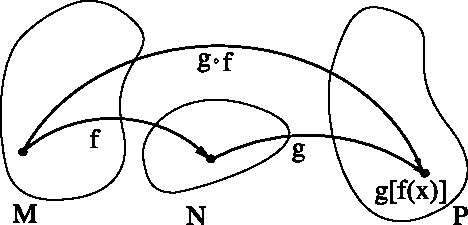
\includegraphics{images/composizione_mappe.pdf}
	\caption[Composition of maps]{Composition of maps. Figura presa da \cite{ferrari2020general}.}
	\labfig{comp_maps}
\end{marginfigure} 
\subparagraph{Composition of mapping}
\hypertarget{map-comp}{Given} two maps \(f : \mathbf{M} \to \mathbf{N}\) and \(g : \mathbf{N} \to \mathbf{P}\), there exists a map $g \circ f$ that maps $\mathbf{M}$ to $\mathbf{P}$
\[
g \circ f : \mathbf{M} \to \mathbf{P}
\]
This means the following: take a point $x \in \mathbf{M}$ and find the image $f(x) \in \mathbf{N}$, then use $g$ to map this point to a point $g(f(\mathbf{x})) \in \mathbf{P}$ (\reffig{comp_maps}).

\begin{definition}[local chart]
A \textbf{local chart}\footnote{We omit the word "local" from now on. A chart is local unless we explicitly say that is global.}\index{Local chart},  or local coordinate system, or local coordinate frame, on a set $M$ is an \underline{\textbf{injective}} map
\[
\varphi: \varphi^{-1}(u)\subseteq \mathbb{R}^n \ \rightarrow \ \underset{\mathclap{\tikz \node {$\uparrow$} node [below=1ex] {\footnotesize Arrival set};}}{u} \subseteq \mathbf{M}
\]
from an \textbf{open}\marginnote[-50 mm]{From \cite{ferrari2020general}: \index{Open set}A set of points $\mathbf{S} \subset \mathbb{R}^n$ is \textit{open} if every point \(x \in \mathbf{S}\) has a neighbourhood entirely
contained in $\mathbf{S}$. This implies that an open set does not include the points on its boundary. For instance, an open ball is an open set; a closed ball, defined by \(\abs{x - y} \leq r\), is not an open set, because the points of the boundary, i.e. \(\abs{x - y} = r\), do not admit a neighbourhood
contained in the set.\\
The open sets of $\mathbb{R}^n$ satisfy the following properties:
\begin{enumerate}
    \item if $\mathbf{O}_1$ and $\mathbf{O}_2$ are open sets, their intersection is also an open set;
    \item the union of any collection (possibly infinite in number) of open sets is open.
\end{enumerate}} subset of $\mathbb{R}^n$ to an open subset of $\mathbf{M}$. The chart is denoted as a pair
\(
\left(u,\varphi\right)
\).
\end{definition}
Let $u$ and $\Tilde{u}$ be two overlapping open sets of $\mathbf{M}$ with two distinct maps from $\mathbb{R}^n$ into a subset of $\mathbf{M}$. The overlap $u\cup\tilde{u}$ is open (since it is the intersection of two open sets), and is given two different coordinate systems by the two maps. Thus, there must exist some relation between these maps, which we want to find.\\
As shown in the lower panel of \reffig{Coordinate-transformation}, pick a point $\mathbf{x}=(x^1,\dots,x^n)$ in the image of the
overlapping region belonging to $\varphi^{-1}(u)$, i.e. $\varphi^{-1}(w)$. Then, use the inverse of the map $\tilde\varphi$, i.e. $\tilde{\varphi}^{-1}$, to go from $p$ to its image belonging to  $\tilde{\varphi}^{-1}(w)$, i.e. to
the point $\tilde{\mathbf{x}}=(\tilde{x}^1,\dots,\tilde{x}^n)$ in $\mathbb{R}^n$,
\[
\tilde{\varphi}^{-1}\circ\varphi: \quad  \underset{\mathclap{\tikz \node {\rotatebox{-90}{$\subseteq$}} node [below=1ex] {\footnotesize $\mathbb{R}^n$};}}{\varphi^{-1}(w)} \to\underset{\mathclap{\tikz \node {\rotatebox{-90}{$\subseteq$}} node [below=1ex] {\footnotesize $\mathbb{R}^n$};}}{\tilde{\varphi}^{-1}(w)}
\]
\begin{marginfigure}
	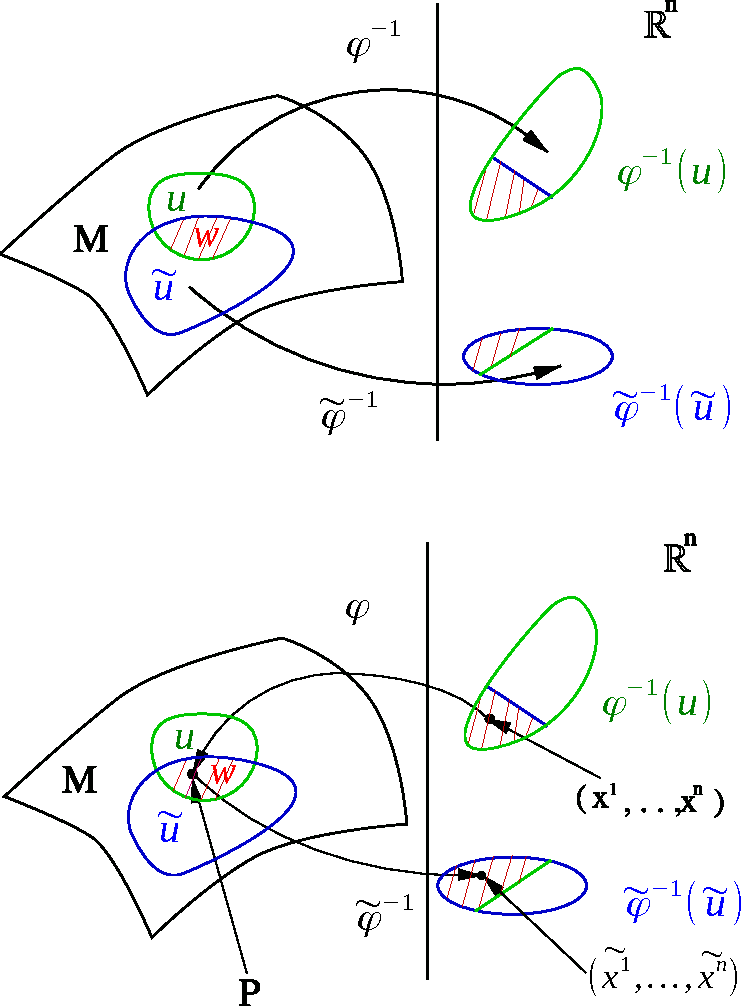
\includegraphics{images/coordinate_change.pdf}
	\caption[Coordinate transformation]{Two overlapping open sets of a manifold, with different maps $\varphi$, $\tilde{\varphi}$ into $\mathbb{R}^n$ (upper panel). Transformation between two coordinate systems (lower panel). Figura adattata da \cite{ferrari2020general}}
	\labfig{Coordinate-transformation}
\end{marginfigure} 
The result of this operation is a functional relation between the two sets of coordinates,
called \textbf{coordinate transformation}\index{Coordinate transformation} between the two charts.
\begin{kaobox}[frametitle=Notation]
We will indicate the coordinate tranformation as
\begin{equation}\label{eq:coord-trans}
\begin{cases}
\mathbf{x}=\mathbf{x}(\tilde{\mathbf{x}})\ \left[=\varphi^{-1}\circ\tilde{\varphi}(\tilde{\mathbf{x}})\right]\\
\tilde{\mathbf{x}}=\tilde{\mathbf{x}}(\tilde{\mathbf{x}})\ \left[=\tilde{\varphi}^{-1}\circ\tilde{\varphi}(\tilde{\mathbf{x}})\right]
\end{cases}
\end{equation}
\end{kaobox}
For a pure mathematician this is an abuse of notation, because we are using the same letter for the variable in the arrival space and for the function. The proper notation is the one between square brackets. Chissene.\\
If the partial derivatives of order $\leq k$ of all the functions $\{\tilde{x}^i\}$ with respect to all $\{x^i\}$ exist and are continuous, then the charts $(u,\varphi)$ and $(\tilde{u},\tilde{\varphi})$ are said to be $C^k$-related.
\begin{marginfigure}
	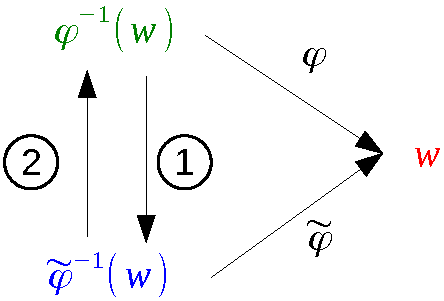
\includegraphics{images/memo_trasf.pdf}
	\caption[Memo coordinate transformation]{Memo for the coordinate transformation}
	\labfig{Memo-Coordinate-transformation}
\end{marginfigure} 
\begin{definition}[Compatibility of charts]\labdef{comp-charts}
Let $\mathbf{M}$ be a set. Two local charts $(u,\varphi)$ and $(\tilde{u},\tilde\varphi)$ are said $\mathbf{C}^\infty-\textrm{\textbf{compatible}}$\footnote{From now one we only say "compatible".} if one of the following happens:
\begin{enumerate}
    \item $u\cap\Tilde{u}=\emptyset \quad$ [unrelated]
    \item \(u\cap\Tilde{u}=w\neq\emptyset\) and it happens that:
    \begin{enumerate}
        \item \(\varphi^{-1}(w)\) and $\tilde{\varphi}^{-1}(w)$ are \textbf{open sets};
        \item the \textbf{change of coordinates}, namely the steps
        \begin{enumerate}
            \item $\varphi^{-1}\circ\Tilde{\varphi}: \quad \Tilde{\varphi}^{-1}(w) \ \rightarrow \ \varphi^{-1}(w)$
            \item $\Tilde{\varphi}^{-1}\circ{\varphi}: \quad {\varphi}^{-1}(w) \ \rightarrow \ \Tilde{\varphi}^{-1}(w)$
        \end{enumerate}
        are $\mathbf{C}^\infty$\textbf{-smooth}.
    \end{enumerate}
\end{enumerate}
\end{definition}
\begin{kaobox}[frametitle=Notice]
Both $\varphi^{-1}\circ\tilde{\varphi}$ and $\tilde{\varphi}^{-1}\circ\varphi$ are maps between \textbf{open subset of $\mathbb{R}^n$}, so we know what $C^\infty$-\href{https://it.wikipedia.org/wiki/Funzione_liscia}{smooth} means: infinitely differentiable (differentiable everywhere, hence continuous, infinitely many times).\marginnote[-4 mm]{Smooth function = "Funzione liscia" in Italian.}
\end{kaobox}
\begin{example}[easy]
Let $\mathbf{M}=\mathbb{R}^2$. Consider two charts:
\begin{enumerate}
    \item \((u,\varphi)=(\mathbb{R}^2, \textrm{ cartesian coordinates})\)
    \item \((\tilde{u},\tilde{\varphi})=(\mathbb{R}^2\setminus\{0\}, \textrm{ cartesian coordinates})\)
\end{enumerate}
Write explicitly $\varphi^{-1}(w)$, $\tilde{\varphi}^{-1}(w)$ and check that $\Tilde{\varphi}^{-1}\circ{\varphi}$ and $\varphi^{-1}\circ\Tilde{\varphi}$ are smooth, hence the charts are compatible.
\end{example}
\begin{definition}[Atlas - Atlante]
An \index{Atlas}\textbf{atlas} for $\mathbf{M}$ is a family of local charts \(\left\{(u_{\alpha},\varphi_{\alpha})\right\}_{\alpha\in A}\) such that one of the following:
\begin{enumerate}
    \item $$\bigcup_{\alpha\in A}u_{\alpha}=\mathbf{M}$$
    \item for every pair $(\alpha,\beta)$ the charts $(u_{\alpha},\varphi_{\alpha})$ and $(u_{\beta},\varphi_{\beta})$ are $\mathbf{C}^{\infty}$ \textbf{-compatible}
\end{enumerate}
\end{definition}
Now we want to define a smooth-Manifold. We could say that is the pair of a set $\mathbf{M}$ equipped with an atlas $A$. The idea is this one, but that is not exactly correct. If we use this definition, we could encounter paradoxes.
\begin{kaobox}[frametitle=Remark]
Atlas on a set $\mathbf{M}$ are naturally \textbf{ordered}\footnote{Ordered, but not "well-ordered" ("\href{https://it.wikipedia.org/wiki/Buon_ordine}{ben ordinato}"), this is why I could arrive to the same maximal atlas from another branch. In general there will be infinitely many branches.}:\\
$A\subseteq \tilde{A}$ if every chart in $A$ is also a chart in $\tilde{A}$ [and henche compatible with every chart in $\tilde{A}\setminus A$]. By abstract results/reasons (\href{https://it.wikipedia.org/wiki/Lemma_di_Zorn}{Zorn's lemma})\marginnote{Zorn's lemma is equivalent to the \href{https://it.wikipedia.org/wiki/Assioma_della_scelta}{axiom of choice }.\\\href{https://it.wikipedia.org/wiki/Lemma_di_Zorn}{Zorn's lemma}:\index{Zorn's lemma} Suppose a partially ordered set $P$ has the property that every chain in $P$ has an upper bound in $P$. Then the set $P$ contains at least one maximal element.}, given $A_0$, there exist a \textbf{maximum element} $A_{\textrm{max}}$, i.e.
\[
\begin{split}
    A_0 \subseteq A_1 \subseteq A_2  \rotatebox{-40}{$\subseteq$}\\
    \tilde{A}_0 \subseteq \tilde{A}_1 \subseteq \tilde{A}_2 \rotatebox{40}{$\subseteq$}
\end{split}
 A_3 \subseteq \dots \subseteq A_{\textrm{max}}
\]
If there exist another maximal atlas, say $B_{\textrm{max}}$, we say that $\mathbf{M}$ admits an \textbf{exotic structure}\index{Exotic structure}.\marginnote[-2mm]{It could exist another family of atlases such that
\[
\begin{split}
    B_0 \subseteq B_1 \subseteq B_2 \rotatebox{-40}{$\subseteq$}\\
    B_\ast \rotatebox{40}{$\subseteq$}
\end{split}
 \dots \subseteq B_{\textrm{max}}
\]
This is the case for \href{https://en.wikipedia.org/wiki/Exotic_R4}{$\mathbb{R}^4$}, but not for $\mathbb{R}^2$ and $\mathbb{R}^3$.}
\end{kaobox}
This $A_{\textrm{max}}$ it is not something we can touch with our hands: it is like the library of all books that has been written and that of those that will be written in the future. We know it exists, but we do not need to describe it. Instead, what we are going to do is to specify a smaller one, and this determines the maximal element. Now we are ready for our definition.\marginnote{{\fontencoding{U}\fontfamily{futs}\selectfont\char 66\relax} You are not really supposed to specify $A$!! You are supposed to \underline{specify an atlas $A_0$}, and $A_0$ determines a corresponding maximal atlas.}
\begin{definition}[Differential manifold - Varietà differenziabile]
A (smooth) \textbf{manifold} \index{Differential manifold} is a pair $(\mathbf{M},A)$ where $\mathbf{M}$ is a set and $A$ is a \underline{\textbf{maximal}} atlas.
\end{definition}
\paragraph{Explanation: Why the hell do we need maximality??}
Why cannot we define a manifold as a set and an atlas? Let us see one of the paradoxes this choice would lead to, looking at this simple non-trivial example represented in \reffig{atlas-circle}: $\mathbf{M}=S^1$
\begin{figure}[H]
	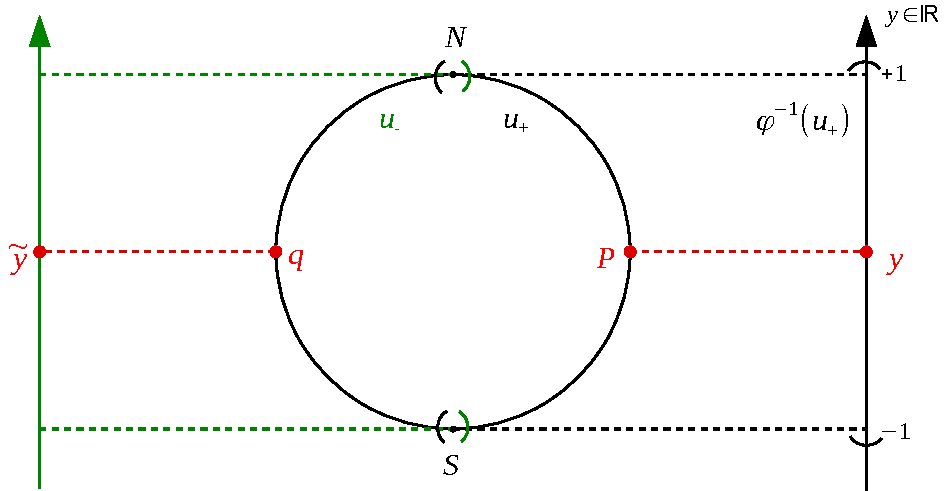
\includegraphics{images/paradox_maximality.pdf}
	\caption[Mapping a circle]{Two possible local charts for a circle. The union of the two covers the circle, except for the poles.}
	\labfig{atlas-circle}
\end{figure} 
\begin{itemize}
    \item Let us choose two arbitrary antipodes points, that we call North (N) and South pole (S);
    \item Let us take open set, which is the East part of the circle
    \item Let us project and associate to the North Pole the value $+1$ and to the South $-1$, this will produce a local chart that associate for every point $y \in (-1,1)$ the point
    \[
    P =
    \begin{pmatrix}
    \sqrt{1-y^2}\\
    y
    \end{pmatrix}
    \]
\end{itemize}
But we can construct another maps in the same way, but using the West part of the circle.\marginnote{We could also use four orthogonal projections: North-West, North-East, South-West, South-East.} This defines an atlas of orthogonal projections:
\[
A_{\textrm{ortho}}:=\left\{\left(u_+,\varphi_+\right), \left(u_-,\varphi_-\right)\right\} \ \textrm{is an atlas on } \mathbf{M}
\]
\begin{figure}[H]
	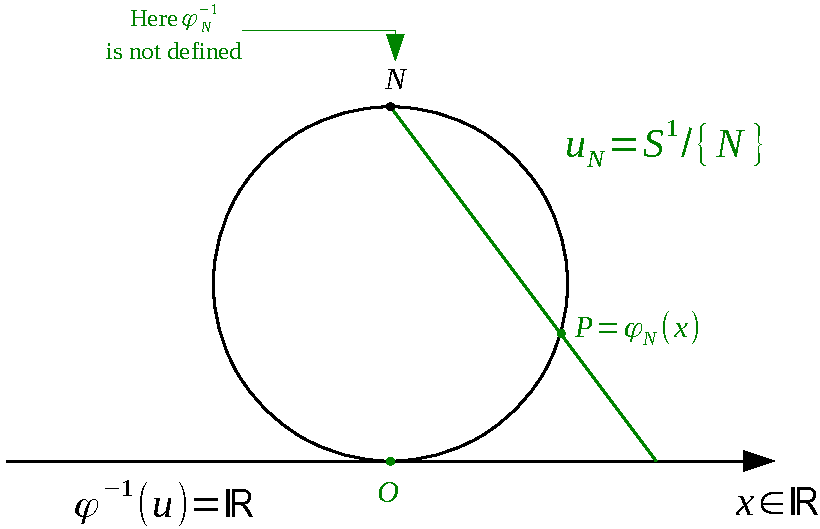
\includegraphics{images/stereo_proj.pdf}
	\caption[Stereographic projection of a circle]{Stereographic projection of a circle}
	\labfig{circle-stereo-proj}
\end{figure} 
But I have another choice that is also very convenient: \textbf{Stereographic projection} from the North Pole, that is represented in \labfig{circle-stereo-proj}
\begin{itemize}
    \item To the North Pole (N) we associate the point $0$ in the local chart, and to the point $x$ a unique point which on the segment from $x$ to $N$.
\end{itemize}
Of course we could to the same from the South Pole.
\[
A_{\textrm{stereo}}:=\left\{\left(u_N,\varphi_N\right), \left(u_S,\varphi_S\right)\right\} \ \textrm{is an atlas on } \mathbf{M}
\]
If we had omitted the reuirement of \textbf{maximality}, we would have that\marginnote{This is not strictly a paradox.}
\[
\begin{rcases}
\left(\mathbf{M},A_{\textrm{ortho}}\right) \ \textrm{is a manifold}\\
\left(\mathbf{M},A_{\textrm{stereo}}\right) \ \textrm{is another manifold} 
\end{rcases}
\textrm{ \fontencoding{U}\fontfamily{futs}\selectfont\char 66\relax} \textrm{ Problem}
\]
Imagine that when we talk about manifold we talk about the two sphere, which one of the two do we need to consider? It is easier to add few lines to our definition ans say that we need to consider the \textit{maximal atlas}, because the mathematical nature of the object is nicer than we might expect, in fact if we take one orthogonal projection and one stereo-graphic projection, on the intersection they are compatible
\[
\begin{split}
    A_{\textrm{ortho}} \rotatebox{-40}{$\subseteq$}\\
    A_{\textrm{stereo}} \rotatebox{40}{$\subseteq$}
\end{split}
 A_{\textrm{ortho}} \cup A_{\textrm{stereo}} \subseteq \dots \underset{\mathclap{\tikz \node {$\uparrow$} node [below=1ex] {\footnotesize \href{https://it.wikipedia.org/wiki/Trasformata_di_Cayley}{Cayley transform}};}}{\subseteq} A_N \subseteq \dots \subseteq A_{\textrm{\textbf{max}}}
\]
\section[Examples of n-dim manifolds]{Examples of n-dimensional manifolds}
\begin{example}
The most trivial example
\[
\mathbf{M}=\mathbb{R}^n \quad A=\left\{\left(\mathbb{R}^n,\mathbb{1}\right)\right\}
\]
\end{example}
\begin{example}
Let us take an open subset $\mathbf{O}\subseteq\mathbb{R}^n$\marginnote{$\mathbb{1}\lceil_{\mathbf{O}}$: the identity is restricted to the copy of $\mathbf{O}$ in the local chart.}
\[
\mathbf{M}=\mathbf{O} \quad A=\left\{\left(\mathbf{O},\mathbb{1}\lceil_{\mathbf{O}}\right)\right\}
\]
\end{example}
\begin{marginfigure}
	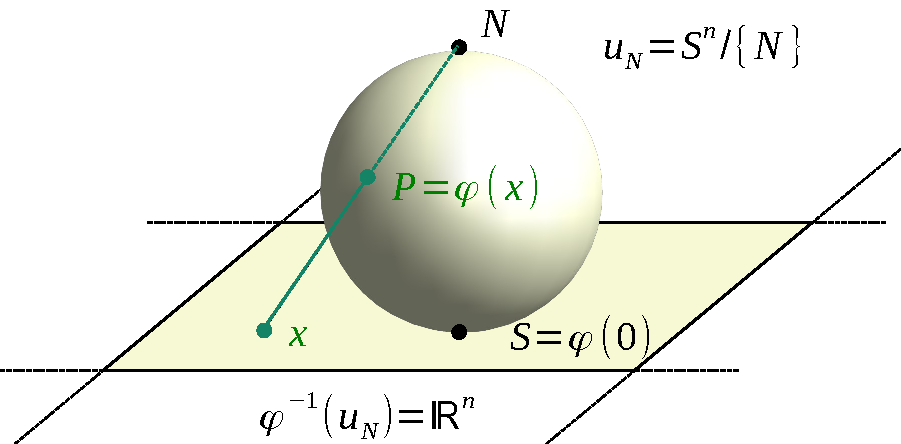
\includegraphics[width=1.1\linewidth]{images/esempio_1_sfera.pdf}
	\caption[Example of n-dim manifold]{Example of n-dim manifold}
	\labfig{Example-n-dim-manifold}
\end{marginfigure} 
\begin{example}\labexercise{sphere}
Let us consider a sphere
\[
S^n=\left\{x\in\mathbb{R}^{n+1}:\ \abs{x}=1\right\}
\]
Let us construct the atlas with the stereo-graphic projections as in \reffig{Example-n-dim-manifold}. Choose two antipodes points $\left\{N,S\right\}$, $u_N$ is the sphere except for the North Pole point. Then we take the atlas of the two stereo-graphic projections\footnote{We omit the checking that they are compatible.}, which is not maximal
\[
A_{\textrm{stereo}}:=\left\{\left(u_N,\varphi_N\right), \left(u_S,\varphi_S\right)\right\} \ \textrm{determines a \textbf{maximal atlas} } A_{\textrm{max}}
\]
\[
\left(S^2,A_{\textrm{max}}\right) \textrm{ is a (smooth) manifold.}
\]
\end{example}
\begin{marginfigure}
	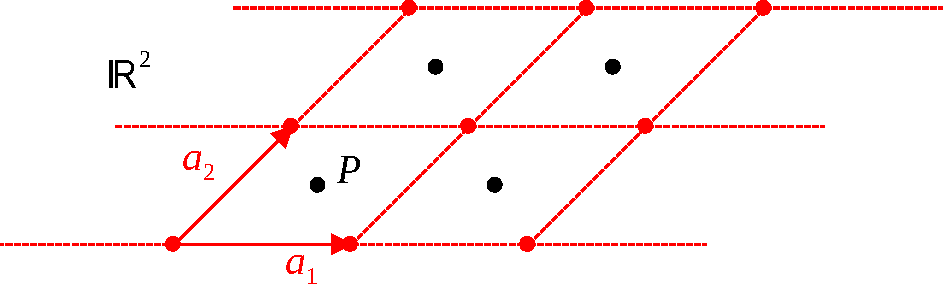
\includegraphics[width=1.1\linewidth]{images/bravais_lattice.pdf}
	\caption[2D bravais lattice]{2D bravais lattice}
	\labfig{bravais-lattice}
\end{marginfigure} 
\begin{marginfigure}
	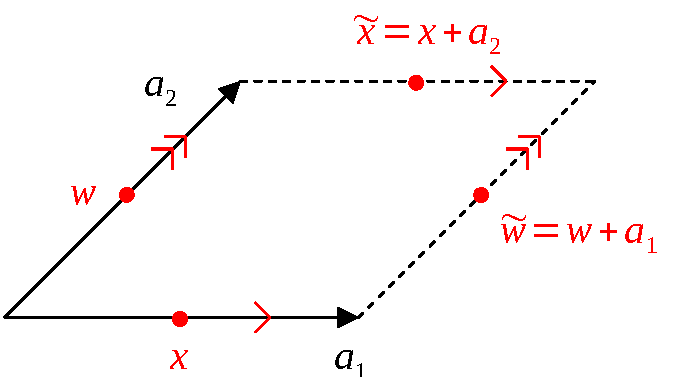
\includegraphics[width=1.1\linewidth]{images/zoom_lattice.pdf}
	\caption[Zoom of the Bravais lattice]{Zoom of the Bravais lattice}
	\labfig{bravais-lattice-zoom}
\end{marginfigure} 
\begin{example}\labexercise{torus}
\textbf{Torus - Toro}: the intrinsic viewpoint\\
This examples is simple, but it shows why sometimes is convenient to use the intrinsic viewpoint. Take $\mathbb{R}^2$ and two linearly independent vectors, not necessarily orthogonal $\mathbf{a_1},\mathbf{a_2}$, as in \reffig{bravais-lattice}. There consider all the points of $\mathbb{R}^2$ that are obtained by taking linear combinations with integer coefficients of these two vectors. This is called a \textbf{Bravais lattice - reticolo di Bravais}.\index{Bravais lattice}
\[
\begin{split}
    \Gamma 
    &= \left\{x\in \mathbb{R}^2: x = n_1a_1+n_1a_2 \ \textrm{for} \ n_1,n_2\in \mathbb{Z}\right\}\\
    &=\textrm{Span}_{\mathbb{Z}}\left\{a_1,a_2\right\}\subseteq\mathbb{R}^2
\end{split}
\]
Now we can take the \textbf{quotient} to identify vectors $x,\tilde{x}\in\mathbb{R}^2$ when differ by a vector $\gamma\in\Gamma$. To be more precise
\[
\textrm{Equivalence relation}: x\sim \tilde{x} \Leftrightarrow \exists \ \gamma \in \Gamma: \tilde{x}=x+\gamma
\]
How many equivalent classes there are? Every point $P$ inside the \href{https://it.wikipedia.org/wiki/Rombo_(geometria)}{rhombus} represent an equivalent class. What about the boundary? We see that the points $x$ and $\tilde{x}$ in \labfig{bravais-lattice-zoom} and in the same equivalent class, since they differ by $a_2$. Therefore the set of equivalent classes is the rhombus, and let us choose to orientate the edges with the same orientation, as represented in the same figure. You may recognise that this is topologically a torus (see \reffig{torus-constr}).\marginnote[-9mm]{This example is inspired by solid state physics.}\marginnote[-1mm]{It depends on gamma, because even if it is always topologically a torus, they can be different tori.}
\[
\textrm{The quotient }\  \mathbb{R}^2/\Gamma =: \Pi^2_{\Gamma} \ \textrm{ is called \textbf{Brillouin torus}}
\]
This is an example of a set which is not canonically embedded in $\mathbb{R}^d$ for some large $d$. \marginnote[-9mm]{The circle was embedded in $\mathbb{R}^2$, and the sphere of the \refexercise{sphere} was embedded in $\mathbb{R}^3$. But the torus of the \refexercise{torus} is not embedded, because is obtained as a quotient.}
\end{example}
\begin{figure*}[h!]
	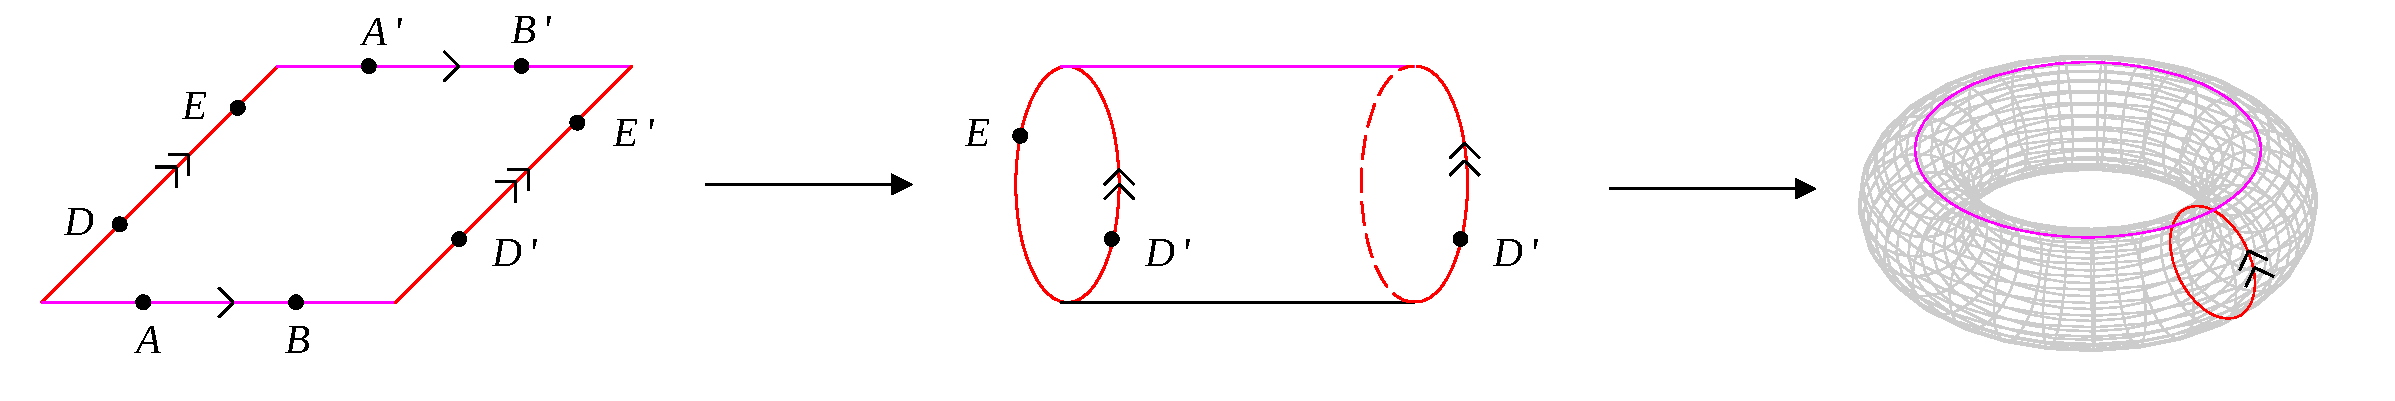
\includegraphics{images/construction_torus.pdf}
	\caption[How to construct a torus]{Visual explanation of why, with an equivalent class, a Brillouin plane is equivalent to a torus. In the last passage we "glued" the two circular edges.}
	\labfig{torus-constr}
\end{figure*}
\begin{example}
Find an atlas of local charts, without embedding $\Pi^2_{\Gamma}$ in some $\mathbb{R}^n$. 
\end{example}
\begin{kaobox}[frametitle=Remark]
The same construction works in $\mathbb{R}^d$ with \[
\Gamma=\textrm{Span}_{\mathbb{Z}}\left\{a_1,a_2,\dots,a_d\right\}
\]
\end{kaobox}
\begin{example}
\textbf{\href{https://it.wikipedia.org/wiki/Bottiglia_di_Klein}{Klein bottle} - Bottiglia di Klein}\index{Klein bottle}\\
We can start again from a square or a rhombus. This time of the two edges is identified with the other with the \textit{opposite} orientation. With this choice you get the figure represented in \reffig{klein-bottle}. There are two procedures to do so:
\begin{enumerate}
    \item You can glue first the purple lines. Then you can bend that and glue them with a \textit{twist}\footnote{You cannot imagine to do that, you need to be in $\mathbb{R}^{\geq 4}$ to visualize it.}.
    \item First you do the twist, and then you glue the two short edges obtaining a Möbius strip - \href{https://it.wikipedia.org/wiki/Nastro_di_M\%C3\%B6bius}{Nastro di Möbius}. Then you can glue them in $\mathbb{R}^4$
\end{enumerate}
\end{example}
\begin{figure*}[h!]
	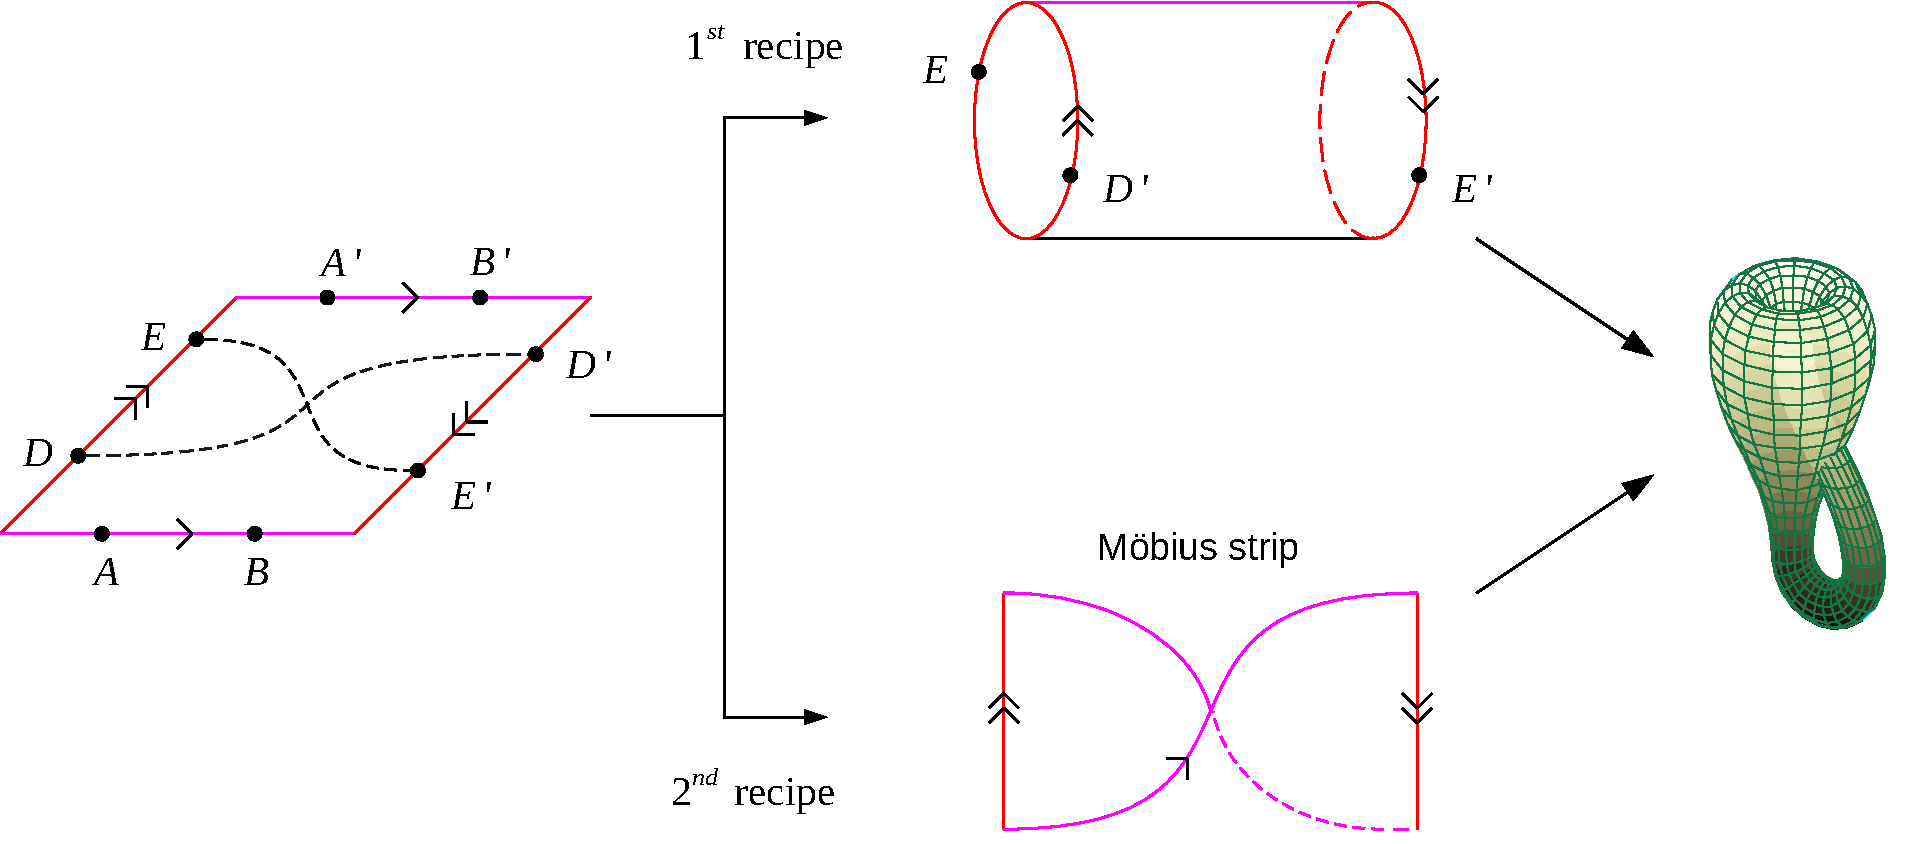
\includegraphics{images/klein_bottle.pdf}
	\caption[How to construct a Klein Bottle]{Two ways to create a Klein bottle. In both cases, to perform the last glueing you need to be in $\mathbb{R}^4$.}
	\labfig{klein-bottle}
\end{figure*}
\begin{example}
(Guided) Do the computations in \sidecite{doCarmo1994} (pages 36-37) to endow the Klein bottle with the structure of a manifold.\marginnote[3mm]{Basically is asking you to define an atlas}
\end{example}
\section[Differentiables maps]{Differentiables maps (functions\sidenote{"Map" and "Function" are synonymous, usually one uses \textit{function} when have values in some numeric field and \textit{map} otherwise.})}
Let (the pair)\sidenote{We will omit the fact that is a pair} $\mathbf{M}=\left(\mathbf{M}, A\right)$ be a manifold. What does it mean that a map $f:\mathbf{M}\to\mathbb{R}$ is $\mathbf{C^\infty}$\textbf{smooth}?
\begin{marginfigure}
	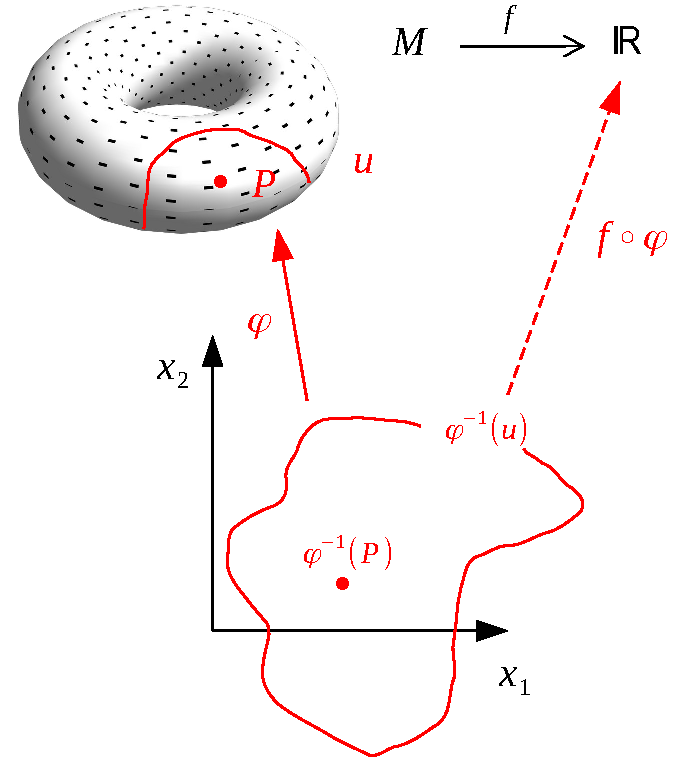
\includegraphics{images/c_smooth.pdf}
	\caption[$C^\infty$-smooth map]{Example of a $C^\infty$-smooth map.}
	\labfig{c-inf-smooth-map}
\end{marginfigure}
\begin{itemize}
    \item Let us take a local chart as in \labfig{c-inf-smooth-map} and we go in the local coordinates $x_1,x_2$, we have a map by composing $f$ and $\varphi$. This is map from an open subset of $\mathbb{R}^n$ to $\mathbb{R}$.
    \item Then we can see that the map $f$ is differential at the point $P$ if the induced map (the local version of  $\varphi$), i.e. $f\circ\varphi$, is differentiable  at the point $\varphi^{-1}(P)$.
    \item This does not depend on the chart, because if we change local chart, the change of coordinates if $C^\infty$-smooth and if we compose two maps that are $C^\infty$-smooth we still get a map which is $C^\infty$-smooth.
\end{itemize}
The trick is that, since all the possible change of coordinates in out maps in the atlas are $C^\infty$-compatible, if it happens that a map is differentiable at $P$ with respect to one local chart, therefore it is differentiable in $P$ with respect to every other local chart in the atlas.
\begin{definition}[Differentiable map]
\index{Differentiables map}A map $f:\mathbf{M}\to\mathbb{R}$ is \textbf{differentiable} (or $\mathbf{C}^\infty$\textbf{-smooth}) at a point $P\in\mathbf{M}$, if for \underline{\textbf{some}} local chart [and, hence, for any other local chart] it happens that $f\circ\varphi: \ \varphi^{-1}(u) \to \mathbb{R}$ is $C^\infty$-smooth at $x=\varphi^{-1}(P)$.\\
We say that the map $f:\mathbf{M}\to\mathbb{R}$ is $\mathbf{C}^\infty$\textbf{-smooth} if it is $C^\infty$-smooth at every point $P\in\mathbf{M}$.
\end{definition}
Similarly we can do the same for a \textbf{continuous} map $f$ (see \refdef{continuous-mapping}) between two manifolds $f:\mathbf{M}\to\mathbf{N}$
\begin{figure}[H]
	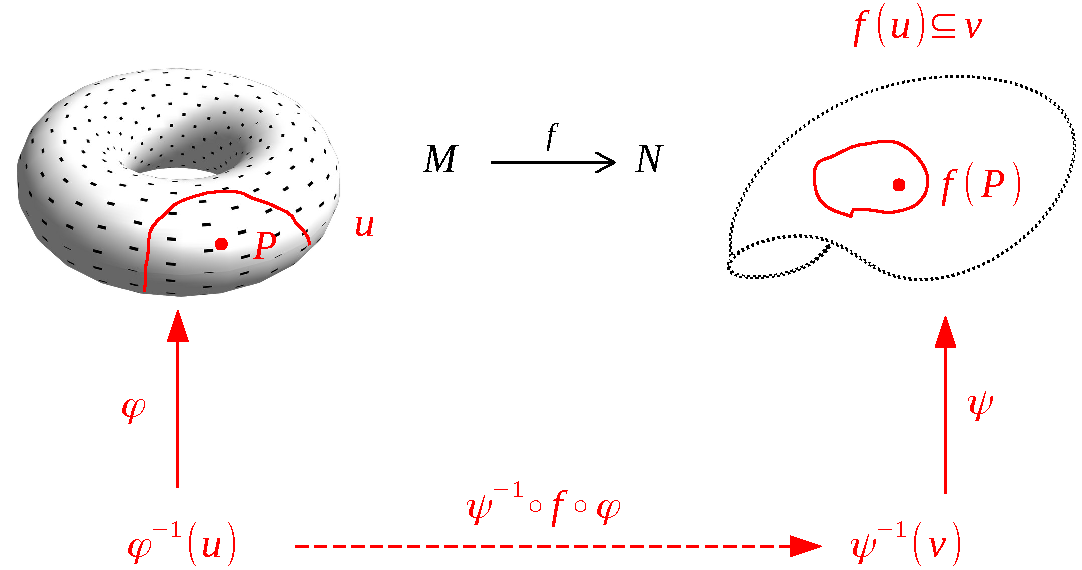
\includegraphics{images/diff_map.pdf}
	\caption[Map between two manifolds]{Map between two manifolds}
	\labfig{map-two-mani}
\end{figure} 
\begin{itemize}
    \item Take a point $p\in\mathbf{M}$, it will have an image $f(P)\in\mathbf{N}$
    \item Now take first a local chart in the arrival space $v$:
    \[ (u,\psi),\ \psi: \psi^{-1}(v)\subseteq \mathbb{R}^n \ \rightarrow \ v \subseteq \mathbf{N}\]
    \item By continuity there exists a local chart in the starting space whose image is completely contained in $v$.\sidenote{Why? Take any local chart that contains $P$ and restrict it up to the point that $u$ is so small that the image of $u$ in inside $v$, i.e. $f(u)\subseteq v$.}
    \item Now take a local chart in the starting space $u$
    \[ (u,\varphi),\ \varphi: \varphi^{-1}(u)\subseteq \mathbb{R}^n \ \rightarrow \ u \subseteq \mathbf{M}\]
    \item Now we can construct the \hyperlink{map-comp}{composition} just by following the arrows
    \[
    \psi^{-1}\circ f\circ\varphi: \quad  \underset{\mathclap{\tikz \node {\rotatebox{-90}{$\subseteq$}} node [below=1ex] {\footnotesize $\mathbb{R}^n$};}}{\varphi^{-1}(u)} \to\underset{\mathclap{\tikz \node {\rotatebox{-90}{$\subseteq$}} node [below=1ex] {\footnotesize $\mathbb{R}^n$};}}{\psi^{-1}(v)}
    \]
\end{itemize}
Since it goes from an open subset of $\mathbb{R}^n$ to an open subset of $\mathbb{R}^n$. We know what it means that is differentiable in this case. Be careful because the fact that the map is differentiable does not depend on the charts we choose (it is intrinsic), but the explicit form of the Jacobian matrix of $f$ does depend. Another intrinsic property is the \textit{rank} of the Jacobian matrix.
\paragraph{The Jacobian \cite{ferrari2020general}}
The notion of differentiable manifold is crucial, because it allows to add “structure” to
the manifold, i.e. to define vectors, tensors, differential forms, Lie derivatives, etc. In order
to complete the definition of coordinate transformation we still need to clarify the following.\\
Let us write equation (\ref{eq:coord-trans}) in the form \[
y^i=f^i(x^1,\dots,x^n) \quad,\quad i=1,\dots,n
\]
where $f^i$ are $C^k$-differentiable. Let $J$ be the Jacobian of the transformation 
\[
J=\frac{\partial(f^1,\dots,f^n)}{\partial(x^1,\dots,x^n)}=\det
\begin{pmatrix}
\frac{\partial f^1}{\partial x^1} & \frac{\partial f^1}{\partial x^2} & \dots & \frac{\partial f^1}{\partial x^n}\\
\frac{\partial f^2}{\partial x^1} & \frac{\partial f^2}{\partial x^2} & \dots & \frac{\partial f^2}{\partial x^n}\\
\vdots & \vdots & \ddots & \vdots\\
\frac{\partial f^n}{\partial x^1} & \frac{\partial f^n}{\partial x^2} & \dots & \frac{\partial f^n}{\partial x^n}
\end{pmatrix}
\]
If $J$ is non-zero at come point $\mathbf{p}$, then the inverse function theorem ensures that the map $f$ is one-to-one in some neighbourhood of $\mathbf{p}$. If $J$ is zero in $\mathbf{p}$ the transformation is singular\index{Singular transformation}.\\
Since a coordinate transformation must be one-to-one in its domain, $J$ must not vanish in this domain.
\begin{definition}[Diffeomorphism - Diffeomorfismo]
Let $\mathbf{M}$ and $\mathbf{N}$ be ($C^\infty-smooth$) manifolds. A \textbf{diffeomorphism} between $\mathbf{M}$ and $\mathbf{N}$ is a bijection
\[
\begin{tikzcd}
\mathbf{M}\rar{f} & \arrow[red, bend left]{l}[black,swap,below]{\color{red}f^{-1}} \mathbf{N}
\end{tikzcd}
\]
such that both $f$ and $f^{-1}$ are $\mathbf{C}^\infty$\textbf{-smooth.}\marginnote{Notice that is not automatic that the inverse is $C^\infty$-smooth, whenever $f$ is. This is in contrast to what happens with linear maps, if we have tow vector spaces and a linear map between them, which is also a bijection, the inverse is automatically linear.}
\end{definition}
\begin{definition}[Diffeomorphic]\index{Diffeomorphoic}
Two manifolds $\mathbf{M}$ and $\mathbf{N}$ are said to be \textbf{diffeomorphic} if there exists a diffeomorphism \(\mathbf{M}\xrightarrow{f}\mathbf{N}\).
\end{definition}
\begin{kaobox}[frametitle=Notation]
We write \(M\cong \mathbf{N}\) or \(M\xrightarrow[f]{\cong}\mathbf{N}\).
\end{kaobox}
\section[Extra]{Extra \sidecite{ferrari2020general}}
With these extra following definitions, it is possible to define a \textit{Manifold} in a more precise way
\begin{marginfigure}
	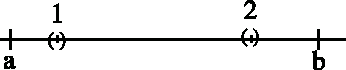
\includegraphics{images/haus_crit.pdf}
	\caption[Representation of Hausdorff’s criterion.]{Representation of Hausdorff’s criterion.}
	\labfig{Hausdorff}
\end{marginfigure} 
\begin{definition}[Hausdorff criterion]
For any two points of a continuum space which do not coincide, there exist two neighbourhoods which do not intersect (see \reffig{Hausdorff})
\end{definition}\labdef{Hausdorff-criterion}
\begin{definition}[Topological space]\index{Topological space}
Let us consider a \textit{general set} $\mathbf{T}$, and a collection of subsets of $\mathbf{T}$, say \(\mathbf{O}=\{\mathbf{O}_i\}\), and call
them \textit{open sets}, such that T itself and the empty set $\emptyset$ belong to the collection. We say that
the pair $(\mathbf{T},\mathbf{O})$, consisting of the set and the collection of subsets, is a topological space, if it satisfies the following properties:
\begin{enumerate}
    \item if $\mathbf{O}_1$ and $\mathbf{O}_2$ are open sets, their intersection is also an open set;
    \item the union of any collection (possibly infinite in number) of open sets is open.
\end{enumerate}
\end{definition}
We remark that the set $\mathbf{T}$ can be any kind of set; the only specification we give is the collection of subsets $\mathbf{O}$, which are by definition the open sets, and that satisfy the properties (1), (2). In particular, in a topological space the notion of distance is a structure which has not been introduced: all definitions only require the notion of open sets. In a topological space $\mathbf{T}$, a neighbourhood $\mathbf{B}(x)$ of a point $x \in \mathbf{T}$ is an open set which
contains the point $x$, i.e. $x \in \mathbf{B}(x)$ and $\mathbf{B}(x) \in \mathbf{O}$. With these definitions, the Hausdorff criterion (and thus the notion of continuum space) can be applied to a topological space: the criterion is satisfied if $\forall x, y \in \mathbf{T}$ such that $x = y$, there exist two neighbourhoods \(\mathbf{B}(x), \ 
\mathbf{B}(y)\) which do not intersect.
\begin{definition}[Continuous mapping]\index{Continuous mapping}\labdef{continuous-mapping}
Given two topological spaces $\mathbf{B}$ and $\mathbf{N}$, a map $f : \mathbf{M} \to \mathbf{N}$ is continuous at $x \in \mathbf{M}$ if any
open set of $\mathbf{N}$ containing $f(x)$ contains the image of an open set of $\mathbf{M}$.
\end{definition}
Finally
\begin{definition}[Manifold]\index{Manifold}
A manifold $\mathbf{M}$ is a topological space, which satisfies the Hausdorff-criterion, and such that each point of $\mathbf{M}$ has an open neighbourhood which has a continuous one-to-one map to an open set of $\mathbb{R}^n$, where $n$ is the dimension of the manifold.
\end{definition}
In this definition we have used the concepts previously defined: the space must be topological, continuous, and we want to associate an n-tuple of real numbers, i.e. a \textit{set of coordinates}, to each point. It should be stressed that the
definition of manifold involves open sets and not the whole $\mathbf{M}$ and $\mathbb{R}^n$, because we do not want to restrict the global topology of $\mathbf{M}$. Moreover, at this stage we only require the map to be one-to-one. We have not yet introduced any geometrical notion such as length, angles, etc.
\newpage
\vspace*{\fill} 
\begin{quote} 
{\centering 
Citation of the day:\\
"Nomina non sunt essentia rerum. Sed nuda nomina tenemus."}\\
\newline
\underline{Free translation}: The coordinates of a point are not the point. However, we need coordinates to compute!
\end{quote}
\vspace*{\fill}
\end{document}